\chapter{Versuch 1 - Bestimmung der Tonhöhe eines akustischen Signals}
\label{chap:VERSUCH_1}


\section{Fragestellung, Messprinzip, Aufbau, Messmittel}
\label{chap:VERSUCH_1_FRAGESTELLUNG}

\subsection*{Fragestellung}
	In diesem Versuch geht es darum einen einzelnen Ton eines Musikinstruments mit einem Mikrofon aufzunehmen.
Das daraus resultierende Signal soll dann in sein Spektrum zerlegt und dargestellt werden.
Dadurch soll ein praktisches Verständnis für die Messung von Tonsignalen und der Fourieranalyse vermittelt werden.
	
\subsection*{Messprinzip}
Die Fourieranalyse ist ein essenzielle Methoden für die Signalverarbeitung. Sie erlaubt es die Grundfrequenz sowie die Obertöne einer Schwingung zu ermitteln.

\subsection*{Aufbau}

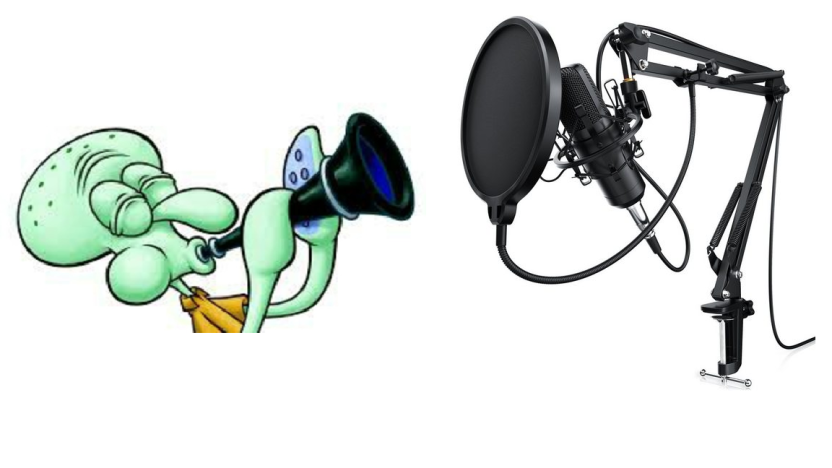
\includegraphics[scale=0.5]{media/Versuchaufbau.png}
\label{Abb:Aufbau}


\subsection*{Messmittel}
\begin{itemize}
	\item Mikrophon
	\item Klanguelle (Klarinette)
\end{itemize}

\section{Messwerte}
\label{chap:VERSUCH_1_MESSWERTE}

Zwei Schwinungen, aus den späteren abschnitten (die ersten 50.000 Werte wurden übersprungen, weil das Signal zu verworren war)
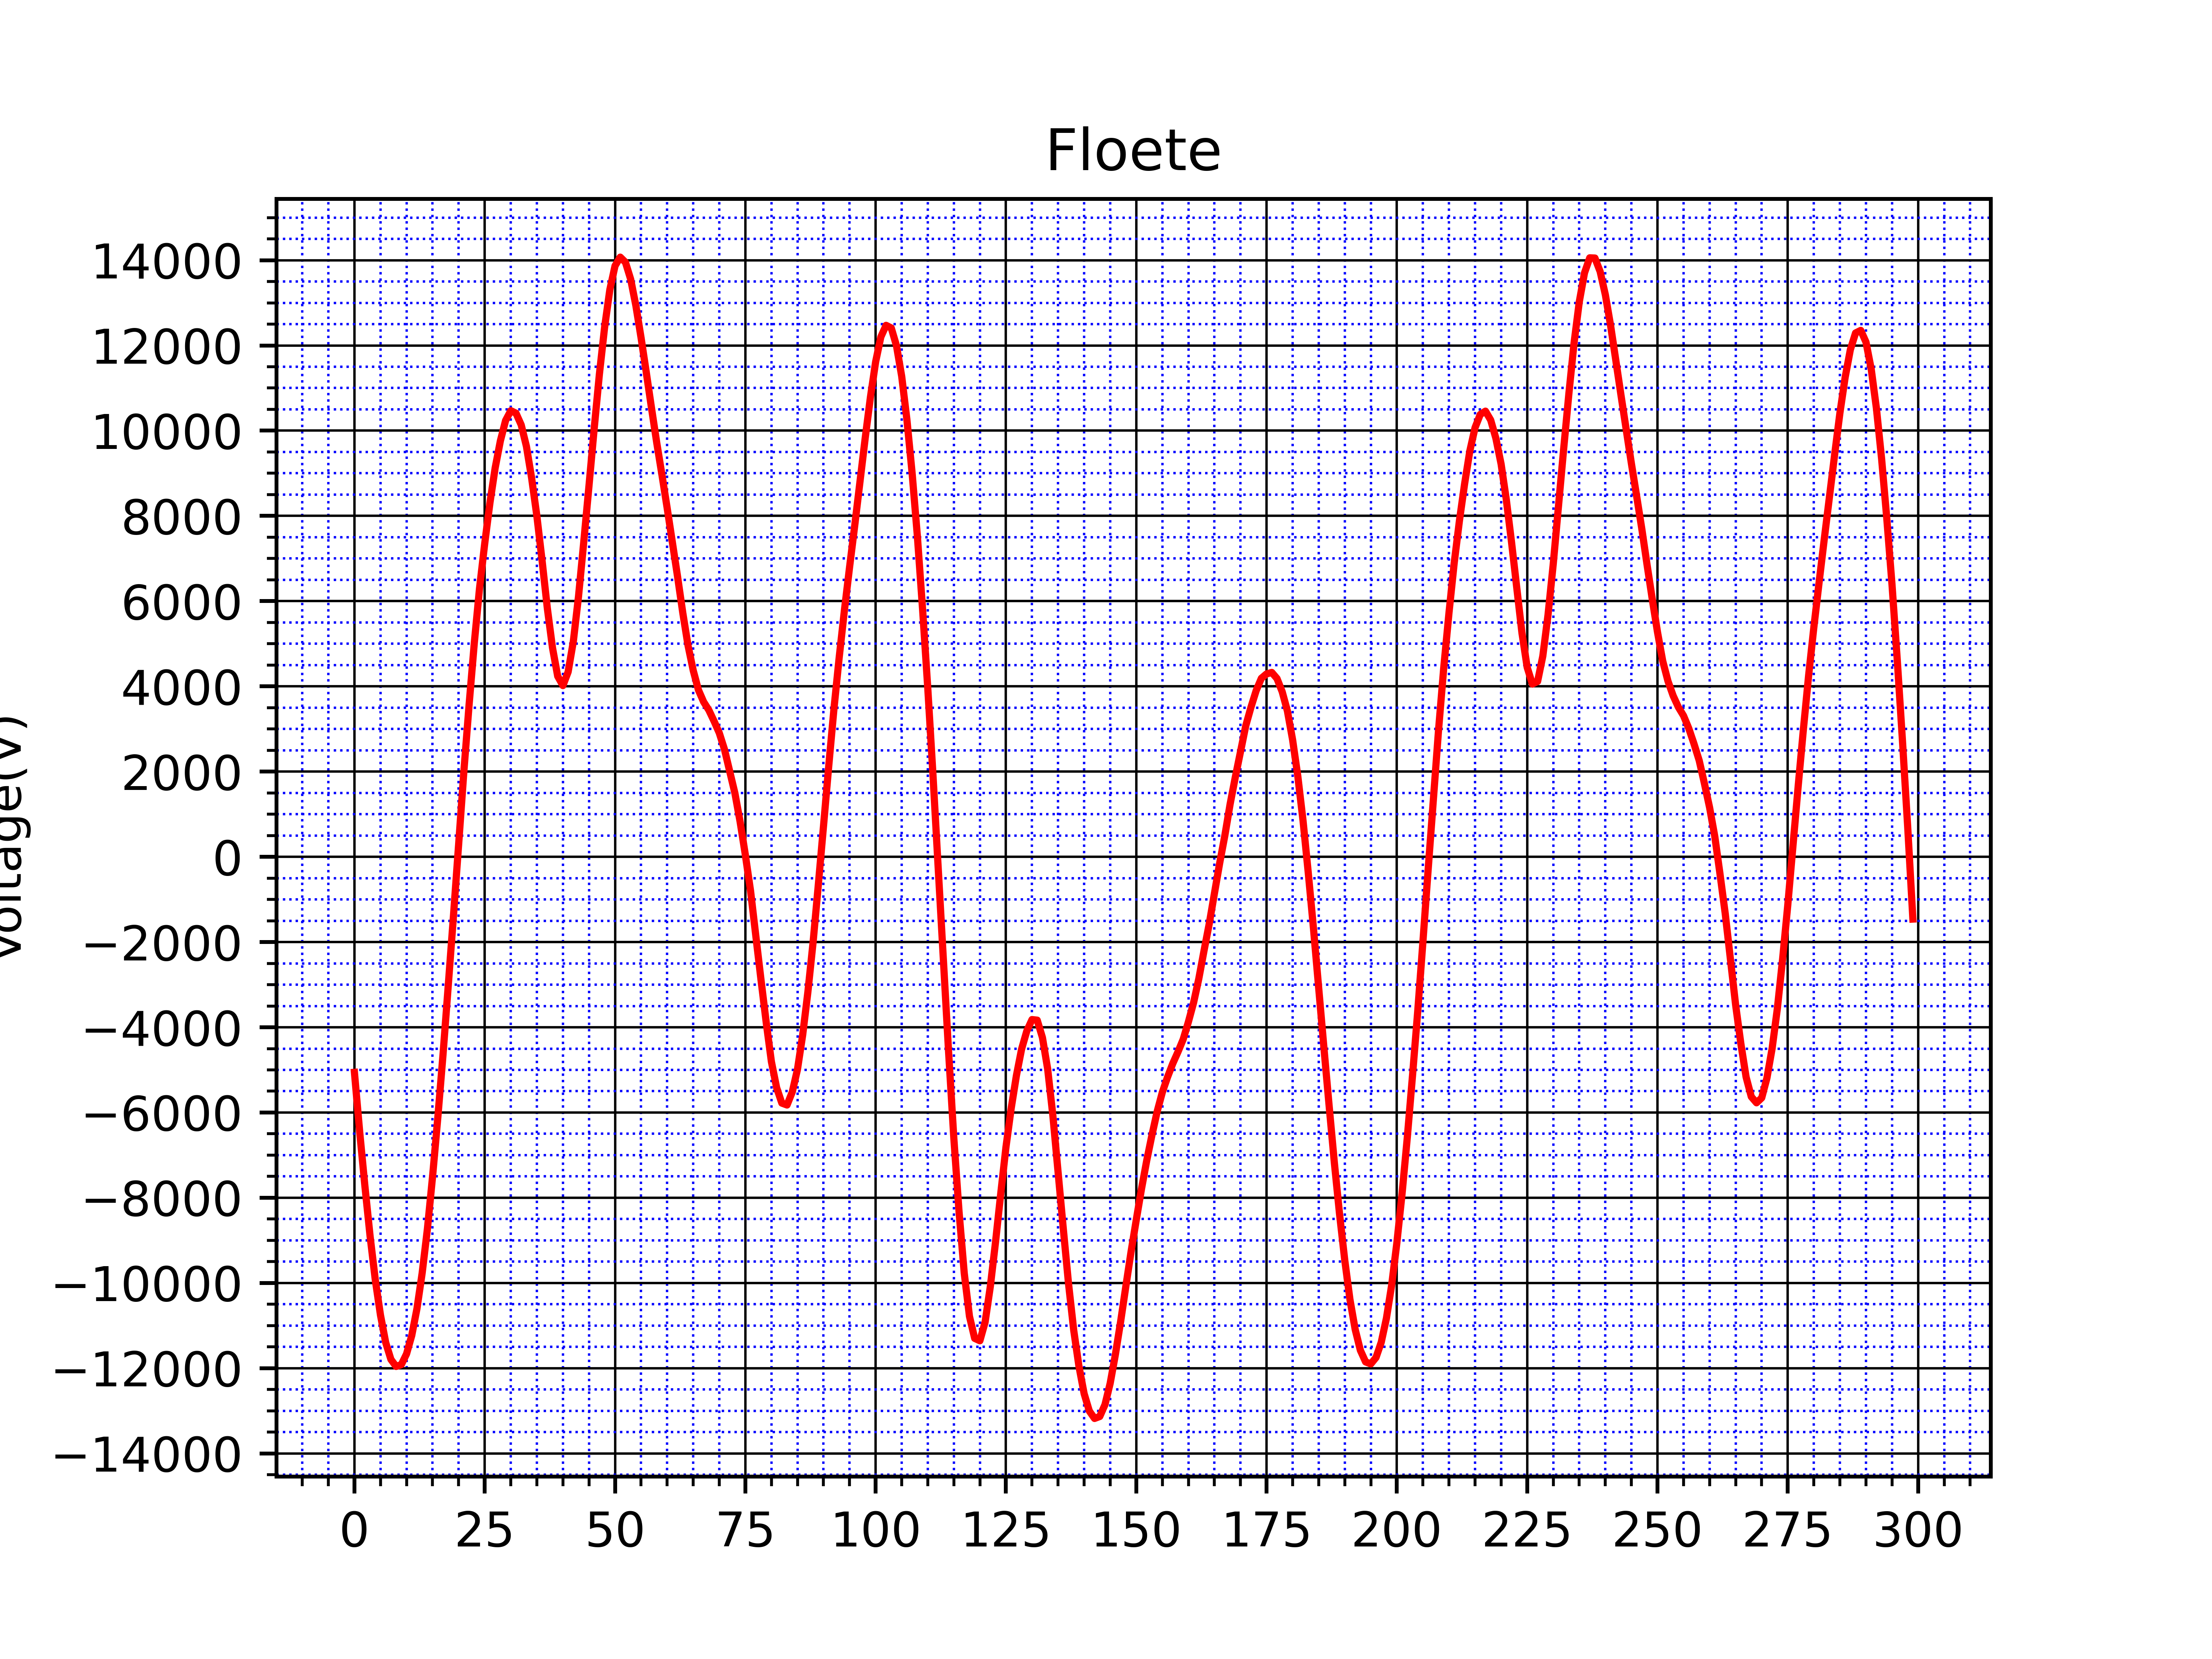
\includegraphics[scale=0.6]{media/Signal_Raster.png}

\section{Auswertung}
\label{chap:VERSUCH_1_AUSWERTUNG}

Zunächst wird die

nun wird die 



\section{Interpretation}
\label{chap:VERSUCH_1_INTERPRETATION}